\documentclass[a4paper, 10pt]{article}

\usepackage[T1]{fontenc}
\usepackage[utf8]{inputenc}
\usepackage[croatian]{babel}
\usepackage{amsmath}
\usepackage{amsfonts}
\usepackage{graphicx} % slike
\usepackage{epstopdf} % eps grafika
\usepackage{listings} % blokovi koda
\usepackage{color}
\usepackage{comment} % blokovi komentara
\usepackage{hyperref}
%\usepackage[nottoc, notbib]{tocbibind} % dodaj popis slika i tablica u toc
\usepackage{lmodern} % sadrži bold stil za tt
\usepackage{afterpage}
%\usepackage{float} % [H] za figure
\usepackage{indentfirst} % indent u prvom paragrafu sekcije
%\setlength{\parindent}{0in} % bez indenta u novom paragrafu
%\setlength{\parskip}{\baselineskip} % razmak između paragrafa

\hypersetup{
  colorlinks = true, % boja linkova
  urlcolor = blue, % boja vanjskih linkova
  linkcolor = black, % boja linkova u dokumentu
  citecolor = red % boja citata
}

%\definecolor{lightgray}{gray}{0.92}

\lstset{
   language = Matlab,
   frame = single,
   %backgroundcolor = \color{lightgray},
   basicstyle = \ttfamily,
   showstringspaces = false,
   showspaces = false,
   breaklines = true,
   inputencoding = utf8, % potrebno za hr slova (listings)
   extendedchars = true, % potrebno za hr slova (listings)
   morekeywords = {ones, mod, randi, rng, saveas}
}

% hrvatska slova u blokovima koda
\lstset{
    literate=%
    {ć}{{\'c}}1
    {č}{{\v{c}}}1
    {đ}{{\dj{}}}1
    {š}{{\v{s}}}1
    {ž}{{\v{z}}}1
    {Ć}{{\'C}}1
    {Č}{{\v{C}}}1
    {Đ}{{\DJ{}}}1
    {Š}{{\v{S}}}1
    {Ž}{{\v{Z}}}1
}

\begin{comment}
\title{Kratki uvod u MATLAB}
\author{Edvin Močibob}
\date{\today}
\end{comment}

\begin{document}

%\maketitle

\begin{titlepage}
\newcommand{\HRule}{\rule{\linewidth}{0.5mm}}
\begin{center}

% Vrh stranice
\textsc{\LARGE Sveučilište u Rijeci}\\[0.5cm]
\textsc{\Large Odjel za informatiku}\\[2.5cm]

% Naslov
\HRule \\[0.4cm]
%{\huge Kratki uvod u MATLAB}\\[0.1cm]
{\huge \bfseries Kratki uvod u MATLAB}\\[0.1cm]

\HRule \\[1.5cm]

% Autor
\begin{minipage}{0.5\textwidth}
	\begin{center}
		\large
		\textsc{\Large Edvin Močibob}\\[0.1cm]
		\texttt{edvin.mocibob@gmail.com}
	\end{center}
\end{minipage}

\vfill
% Dno stranice
{\large \today}
\end{center}
\end{titlepage}

\newpage\null\thispagestyle{empty}\addtocounter{page}{-1}\newpage % prazna stranica

\tableofcontents
\clearpage

\section*{Uvod}
\addcontentsline{toc}{section}{Uvod}

Slijedi kratki uvod u sintaksu MATLAB-a prezentiran (većinom) kroz primjere. Navedeni primjeri testirani su u MATLAB verziji R2014a na Windows 7 operacijskom sustavu. MATLAB ima kvalitetnu dokumentaciju sa primjerima te preporučeno je njezino korištenje uz ovaj dokument.

Kontaktiranje autora u vezi grešaka u tekstu i unaprjeđenja sadržaja preko email adrese na naslovnoj stranici.

\clearpage

\section{Osnove}

Jednolinijski komentari počinju sa \texttt{\%}.

\begin{lstlisting}
x = 5 % varijabla x poprima vrijednost 5
\end{lstlisting}

Spremanje radne površine (\textit{workspace}) pomoću \texttt{save}.

\begin{lstlisting}
save('vjezba1_data')
\end{lstlisting}

Generiranje vektora koji sadrži $4$ vrijednosti koje idu od $1$ do $10$ (granice uključne). Sve susjedne vrijednosti su međusobno jednako udaljene.

\begin{lstlisting}
linspace(1, 10, 4) % rezultat sadrži 1, 4, 7 i 10
\end{lstlisting}

Isti rezultat dobijemo sljedećom naredom. Ovdje ne odredimo eksplicitno broj elementa nego inkrement za svaki sljedeći element (u ovom slučaju $3$).

\begin{lstlisting}
[1:3:10]
\end{lstlisting}

Sa istim operatorom moguće je potencirati i pojedinačne brojeve i vektore (matrice).

\begin{lstlisting}
a = 5
b = [1, 2, 3, 4]
a .^ 3
b .^ 3
\end{lstlisting}

Duže naredbe je zbog preglednosti moguće napisati u više linija sa tri točke.

\begin{lstlisting}
n = 1 - 1/12 + 1/123 - 1/1234 + 1/12345 - 1/123456 ...
       + 1/1234567 - 1/12345678 + 1/123456789
\end{lstlisting}

Izlaz naredbe neće se prikazati ako naredba završi sa \texttt{;}.

Trenutni radni prostor može se obrisati narednom \texttt{clear}, dok \texttt{clc} služi za brisanje sadržaja komandne linije.

\section{Matrice}

$2 \times 3$ matrica koja sadrži samo jedinice.

\begin{lstlisting}
ones(2, 3)
\end{lstlisting}

Matrica $A$ sa tri redaka i četiri stupaca.

\begin{lstlisting}
A = [1 2 3 4; 10 20 30 40; 100 200 300 400]
\end{lstlisting}

Transponiranje $A$.

\begin{lstlisting}
A'
\end{lstlisting}

Zbroj elemenata $A$ po stupcima.

\begin{lstlisting}
sum(A) % izlaz 1x4 matrica
\end{lstlisting}

Zbroj svih elemenata.

\begin{lstlisting}
sum(sum(A))
\end{lstlisting}

Najveći element iz $A$.

\begin{lstlisting}
max(max(A))
\end{lstlisting}

Najmanji elementi iz pojedinih redaka.

\begin{lstlisting}
min(A, [], 2)
\end{lstlisting}

Matrica koja sadrži koji elementi $A$ su veći od $30$. Izlaz ima iste dimenzije kao $A$; na mjesta elemenata većih od $30$ nalazi $1$, na ostalim $0$.

\begin{lstlisting}
A > 30
\end{lstlisting}

Broj elemenata $A$ većih od $30$.

\begin{lstlisting}
sum(sum(A > 30))
\end{lstlisting}

Vrati matricu $P$ koja sadrži na kojim mjestima u $A$ se nalaze parni brojevi. Nakon toga ispiši te parne brojeve iz $A$.

\begin{lstlisting}
P = mod(A, 2) == 0;
A(P)
\end{lstlisting}

Matrica $B$ koja sadrži elemente $A$ povećane za $10$.

\begin{lstlisting}
B = A + 10
\end{lstlisting}

Pojedinim elementima $A$ možemo pristupiti sa \texttt{A(i, j)} gdje je \texttt{i} redak a \texttt{j} stupac elementa. Numeriranje za retke i stupce počinje od $1$.

\begin{lstlisting}
A(2, 1) % element u drugom retku i prvom stupcu
\end{lstlisting}

Vrati prvo drugi redak iz $A$, a zatim treći i četvrti stupac.

\begin{lstlisting}
A(2, :)
A(:, 3:4)
\end{lstlisting}

Uvećaj treći stupac 10 puta.

\begin{lstlisting}
A(:, 3) = A(:, 3) * 10;
\end{lstlisting}

Dodaj novi redak na $A$ (trenutne dimenzije $3 \times 4$). Moguće koristiti i \texttt{vertcat}.

\begin{lstlisting}
[A; -1 -2 -3 -4]
\end{lstlisting}

Dodaj novi stupac na $A$ (trenutne dimenzije $3 \times 4$). Moguće koristiti i \texttt{horzcat}.

\begin{lstlisting}
[A [5; 55; 555]]
\end{lstlisting}

Napravi jediničnu matricu (jedinice na dijagonali) $B$ istih dimenzija kao $A$.

\begin{lstlisting}
B = eye(size(A))
\end{lstlisting}

Napravi i zatim matrično pomnoži matrice $C$ i $D$.

\begin{lstlisting}
C = [1 2; 3 4];
D = [10 20; 30 40];
C * D
\end{lstlisting}

Množenje matrica $C$ i $D$ po elementima.

\begin{lstlisting}
C .* D
\end{lstlisting}

\section{Polja ćelija (cell arrays)}

Matrice ne mogu sadržavati istovremeno različite tipove podataka (npr.\ brojeve i tekst). Kada imamo potrebu za nečim takvim možemo koristiti polja ćelija.

Inicijaliziacija se može vršiti pomoću vitičastih zagrada. Što se dimenzija tiče, svi reci moraju imati isti broj elemenata. U primjeru vidimo da polja ćelija mogu sadržavati druga polja ćelija.

\begin{lstlisting}
C = {'Tekst', 2, {'XYZ', 111}; 4, 5, 10}
\end{lstlisting}

Referenciranje ćelija moguće je pomoću uglatih zagrada (gdje se pristupa ćelijama) ili pomoći vitičastih zagrada (gdje se pristupa sadržaju ćelija). U primjeru pristupamo drugom retku polja $C$. 

\begin{lstlisting}
a = C(2, :)
b = [C{2, :}]
\end{lstlisting}

Prazna ćelija dimenzija $0 \times 0$ može se inicijalizirati na sljedeći način.

\begin{lstlisting}
C2 = {}
\end{lstlisting}

Slijedi primjer u kojem se dodaje element u postojeće polje ćelija. Dimenzije polja će se automatski povećati ako se referencira ćelija izvan postojećih dimenzija.

\begin{lstlisting}
C2{4, 4} = 9
\end{lstlisting}

Samo povećanje dimenzija bez dodavanja ikakve nove vrijednosti vrši se na sljedeći način.

\begin{lstlisting}
C2{5, 6} = []
\end{lstlisting}

Naredba \texttt{cell2mat} može se koristiti za pretvaranje polja ćelija (ili samo djela polja ćelija) u obični vektor tj.\ matricu. Uvjet je da svi elementi koji se pretvaraju budu istog tipa.

\section{Petlje}

Ispiši \texttt{for} petljom brojeve od $1$ do $10$ (granice uključne).

\begin{lstlisting}
for i = 1:10
    i
end
\end{lstlisting}

Ista stvar u \texttt{while} petlji.

\begin{lstlisting}
i = 1;
while i <= 10
    i
    i = i + 1;
end
\end{lstlisting}

Ispiši \texttt{for} petljom svaki drugi broj od $1$ do $10$ (tj. ispiši $1$, $3$, $5$, $7$ i $9$).

\begin{lstlisting}
for i = 1:2:10
    i
end
\end{lstlisting}

Napravi matricu $A$ dimenzija $3 \times 4$ i zatim u petlji povećaj svaki njezin element za 10.

\begin{lstlisting}
A = [1 2 3 4; 10 20 30 40; 100 200 300 400]
for i = 1:3
    for j = 1:4
        A(i, j) = A(i, j) + 10;
    end
end
A
\end{lstlisting}

\section{Pseudo-slučajni brojevi}

Generiraj broj između $0$ i $1$.

\begin{lstlisting}
rand
\end{lstlisting}

Generiraj $2 \times 2$ slučajnu matricu sa vrijednostima između $0$ i $1$. 

\begin{lstlisting}
rand(2, 2)
\end{lstlisting}

Generiraj cijeli broj u rasponu od 10 do 20 (granice uključne).

\begin{lstlisting}
randi([10, 20], 1)
\end{lstlisting}

Napravi matricu $A$ dimenzija $5 \times 5$ koja sadrži cijele slučajne brojeve u rasponu od $-100$ do $100$.

\begin{lstlisting}
A = randi([-100, 100], 5, 5)
\end{lstlisting}

Ako želimo da funkcije koje koriste slučajne vrijednosti uvijek daju isti rezultat potrebno je postaviti konstantan \textit{seed} (nenegativni cijeli broj) za generator slučajnih vrijednosti. To činimo pomoću \texttt{rng}.

\begin{lstlisting}
rng(999)
\end{lstlisting}

\section{Stringovi i ispis teksta}

Novi string.

\begin{lstlisting}
s = 'Neki tekst'
\end{lstlisting}

Duljina stringa.

\begin{lstlisting}
length(s)
\end{lstlisting}

Provjeri ako je \texttt{s} string.

\begin{lstlisting}
isstr(s)
\end{lstlisting}

Broj u string.

\begin{lstlisting}
num2str(125)
\end{lstlisting}

String u broj.

\begin{lstlisting}
x = str2num('521')
\end{lstlisting}

Konkatenacija stringova.

\begin{lstlisting}
tekst = [s, ' i na primjer broj ', num2str(125), '.']
\end{lstlisting}

Stringove možemo ispisivati sa \texttt{disp}. Istu funkciju možemo koristiti i na brojevima.

\begin{lstlisting}
disp(tekst)
disp(7)
\end{lstlisting}

Za ispise gdje se kombiniraju različiti formati (stringovi, cijeli i decimalni brojevi itd.) može se koristiti \texttt{fprintf}.

\begin{lstlisting}
fprintf('Umjesto %f koristimo %d\n', 5.67, 5)
fprintf('String od prije glasi: %s\n', tekst)
\end{lstlisting}

\section{Korisnički definirane funkcije}

Primjer funkcije koje ne vraća vrijednost.

\begin{lstlisting}
function parnost(n)
if mod(n, 2) == 0
    disp('Broj paran.')
else
    disp('Broj neparan.')
end
end
\end{lstlisting}

Primjer kada funkcija vraća vrijednost. Konkretno, vrijednost koja se vraća je \texttt{b}.

\begin{lstlisting}
function b = kvadriraj(a)
b = a * a;
end
\end{lstlisting}

Funkcije mogu odjednom vraćati više vrijednosti.

\begin{lstlisting}
function [b, c] = kvadrat_i_kub(a)
b = a * a;
c = b * a;
end
\end{lstlisting}

Prethodno navedenu funkciju bi pozivali na primjer ovako.

\begin{lstlisting}
[kv, kub] = kvadrat_i_kub(11)
\end{lstlisting}

Korisnički definirane funkcije možemo spremati u datoteke sa nastavkom \texttt{.m}.

\section{Korisnički unos}

Korisnika se može tražiti unos na sljedeći način. U primjeru unos se sprema u \texttt{x}.

\begin{lstlisting}
x = input('Unesite broj: ')
\end{lstlisting}

Složeniji upit za unos (u kojem ispisujemo neke varijable) možemo postići na sljedeći način.

\begin{lstlisting}
fprintf('Nova vrijednost (prijašnja %d): ', x)
x = input('')
\end{lstlisting}

Osim brojčanih, moguć je unos i tekstualnih vrijednosti.

\begin{lstlisting}
odg = input('Unesite ime: ', 's')
\end{lstlisting}

\section{Grafovi}

Ovako bi jednostavno nacrtali funkciju sinus na intervalu od $-5$ do $5$. Ako imamo samo jedan graf \texttt{figure} nije obavezan. Rezultat bi trebao izgledati kao slika \ref{fig:plot_sin_1} u prilozima na stranici \pageref{sec:prilozi}.

\begin{lstlisting}
x = linspace(-5, 5, 101);
figure % otvara novi prozor za graf
plot(x, sin(x))
\end{lstlisting}

Sljedeći kod pokazuje kako učiniti da se prozor sa grafom ne otvori. Dodatno, graf se još spremi kao slika pod imenom \texttt{sinus\_graf.png}.

\begin{lstlisting}
x = linspace(-5, 5, 101);
fig = figure('visible', 'off');
plot(x, sin(x))
saveas(fig, 'sinus_graf', 'png')
\end{lstlisting}

Na jednom grafu možemo imati više funkcija odjednom. To radimo tako da jednostavno navodimo argumente svake funkcije jedan za drugim. U donjem primjeru korišteni su i argumenti za stiliziranje linija (\texttt{g} i \texttt{b} su boje, a \texttt{-{}-} i \texttt{:} vrste linija). Rezultat slika \ref{fig:plot_sin_cos_1}.

\begin{lstlisting}
x = linspace(-5, 5, 101);
figure
plot(x, sin(x), 'g--', x, cos(x), 'b:')
\end{lstlisting}

Isti rezultat (slika \ref{fig:plot_sin_cos_1}) moguće je dobiti korištenjem naredbe \texttt{hold}.

\begin{lstlisting}
x = linspace(-5, 5, 101);
figure
plot(x, sin(x), 'g--')
hold on
plot(x, cos(x), 'b:')
\end{lstlisting}

Slijedi primjer sa (detaljnijim) stiliziranjem linije i točaka grafa. Slika \ref{fig:plot_stil}.

\begin{lstlisting}
x = linspace(-5, 5, 21);
y = x .* x;
figure
plot(x, y, '--go', ... % stil linije i oblik točke
    'LineWidth', 2, ... % debljina linija
    'MarkerSize', 6, ... % veličina točke
    'MarkerEdgeColor', 'r', ... % boja ruba točke
    'MarkerFaceColor', 'w') % unutrašnja boje točke
\end{lstlisting}

Naslov grafa, oznake osi i legendu možemo dodati sljedećim kodom. Rezultat slika \ref{fig:plot_sin_cos_oznaceno}.

\begin{lstlisting}
x = linspace(-5, 5, 101);
figure
plot(x, sin(x), 'g--', x, cos(x), 'b:')
title('Vrijednost sin(x) i cos(x) na [-5, 5]')
xlabel('Os x')
ylabel('Vrijednost funkcije')
legend('sin(x)', 'cos(x)')
\end{lstlisting}

MATLAB podržava više vrsta grafova. U sljedećem primjeru prikazan je još stupčasti graf koji vizualizira neke \textit{random} podatke. Naslov grafa, oznake osi itd.\ bi se po potrebi postavile kao za \texttt{plot}. Izlaz slika \ref{fig:bar_1}.

\begin{lstlisting}
rng(999) % postavljenje seed-a za random brojeve
x = 1500:20:1620;
podaci = randi([1, 100], 1, 7);
figure
bar(x, podaci)
\end{lstlisting}

U sljedećem primjeru prikazano je kako se može proizvoljno imenovati svaki stupac. Rezultat slika \ref{fig:bar_imenovan}.

\begin{lstlisting}
rng(999)
podaci = randi([1, 100], 1, 7);
stupci = {'A'; 'B'; 'C'; 'D'; 'E'; 'F'; 'G'};
figure
bar(podaci)
set(gca, 'xticklabel', stupci)
\end{lstlisting}

\clearpage

\section*{Prilozi}
\label{sec:prilozi}
\addcontentsline{toc}{section}{Prilozi}

\begin{figure}[!htb]
\centering
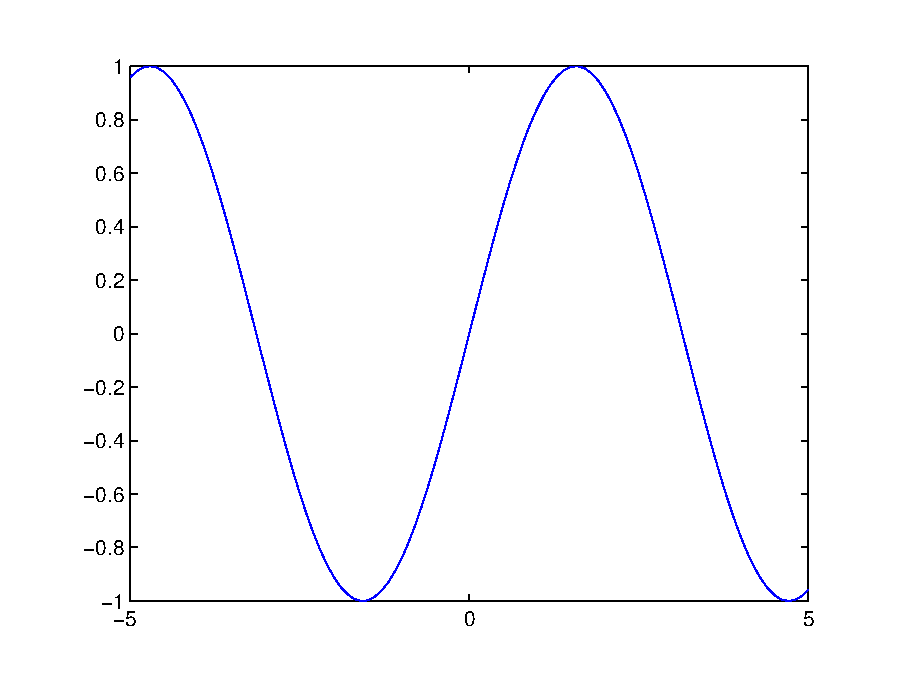
\includegraphics[width=\linewidth]{slike/plot_sin_1.eps}
\caption{Graf funkcije sinus na intervalu $[-5, 5]$.}
\label{fig:plot_sin_1}
\end{figure}

\begin{figure}[!htb]
\centering
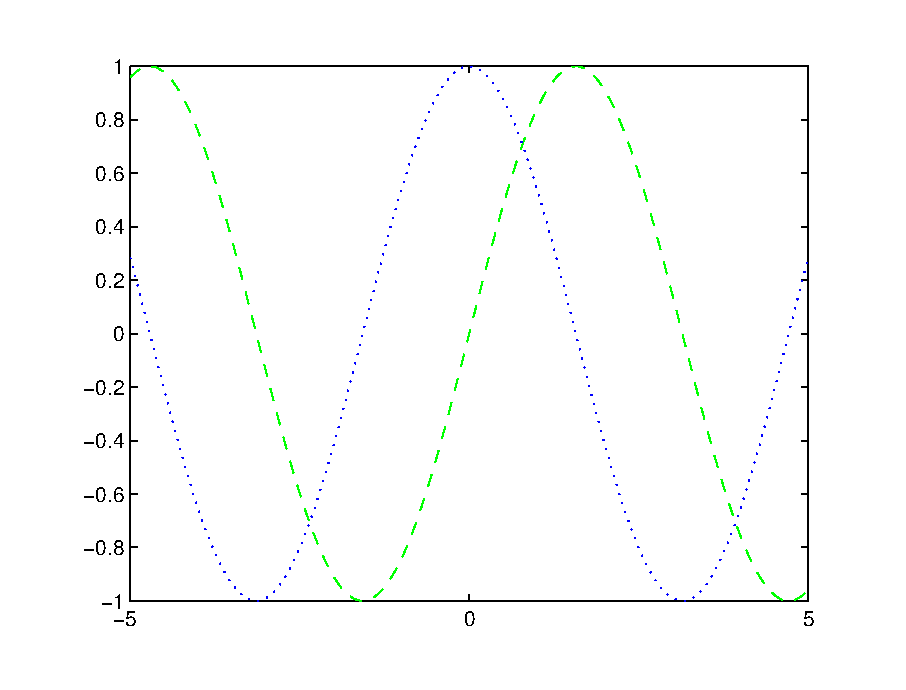
\includegraphics[width=\linewidth]{slike/plot_sin_cos_1.eps}
\caption{Graf funkcija sinus i kosinus na intervalu $[-5, 5]$.}
\label{fig:plot_sin_cos_1}
\end{figure}

\begin{figure}[!htb]
\centering
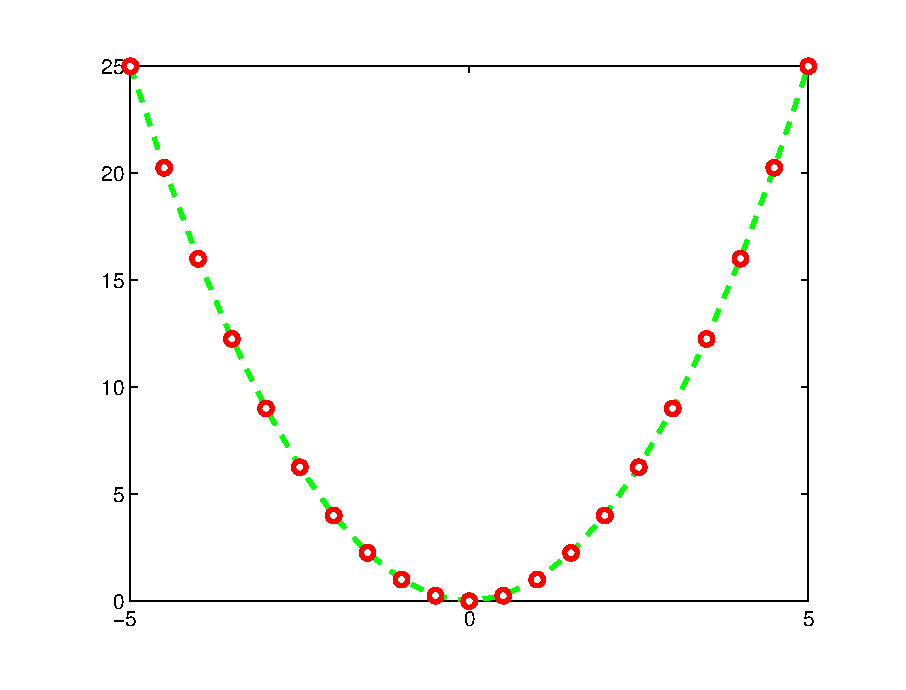
\includegraphics[width=\linewidth]{slike/plot_stil.eps}
\caption{Primjer stiliziranog grafa.}
\label{fig:plot_stil}
\end{figure}

\begin{figure}[!htb]
\centering
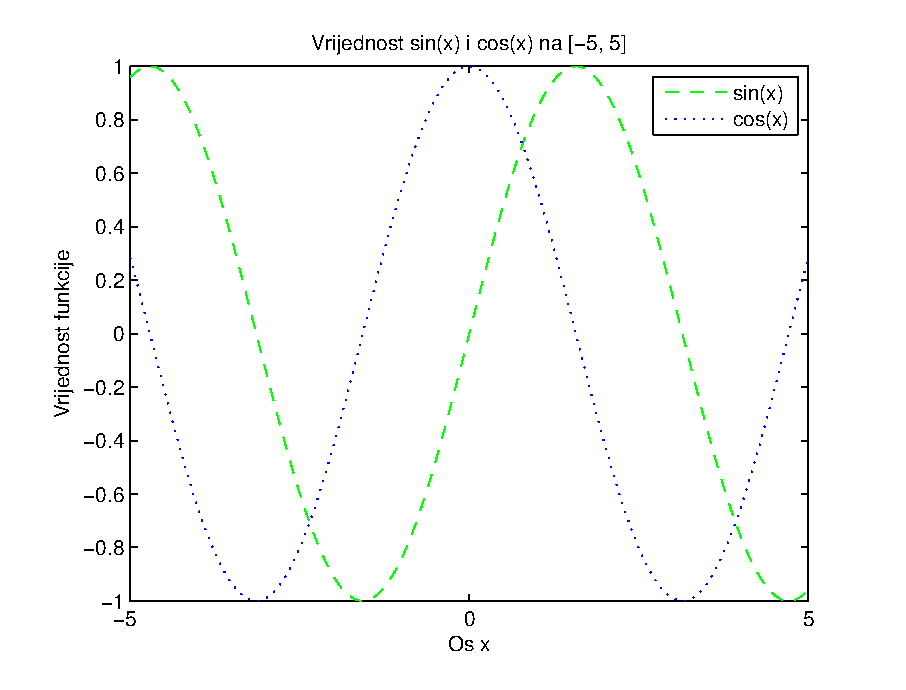
\includegraphics[width=\linewidth]{slike/plot_sin_cos_oznaceno.eps}
\caption{Označeni graf funkcija sinus i kosinus na intervalu $[-5, 5]$.}
\label{fig:plot_sin_cos_oznaceno}
\end{figure}

\begin{figure}[!htb]
\centering
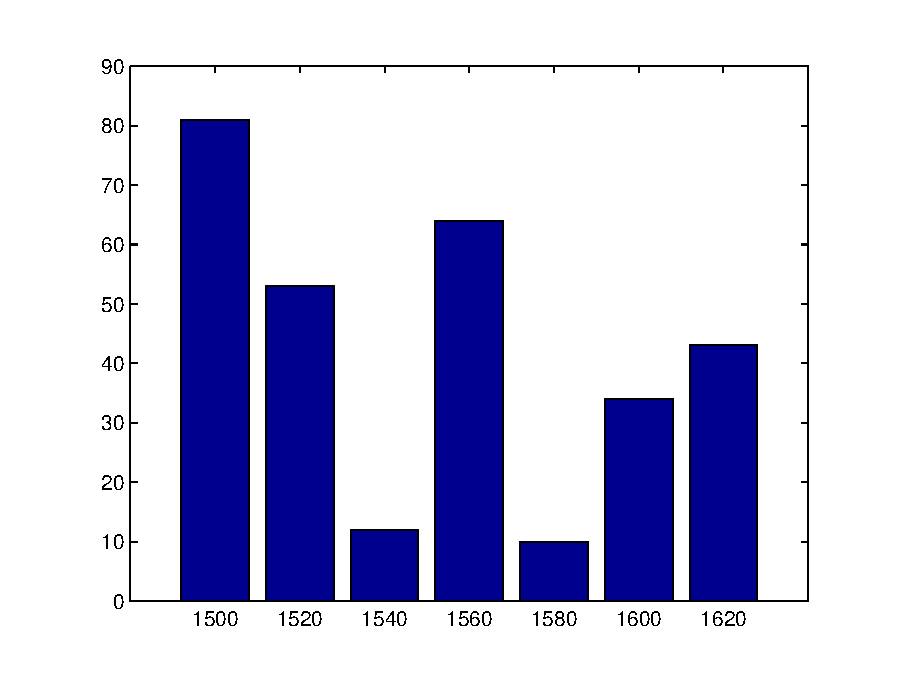
\includegraphics[width=\linewidth]{slike/bar_1.eps}
\caption{Primjer stupčastog grafa.}
\label{fig:bar_1}
\end{figure}

\begin{figure}[!htb]
\centering
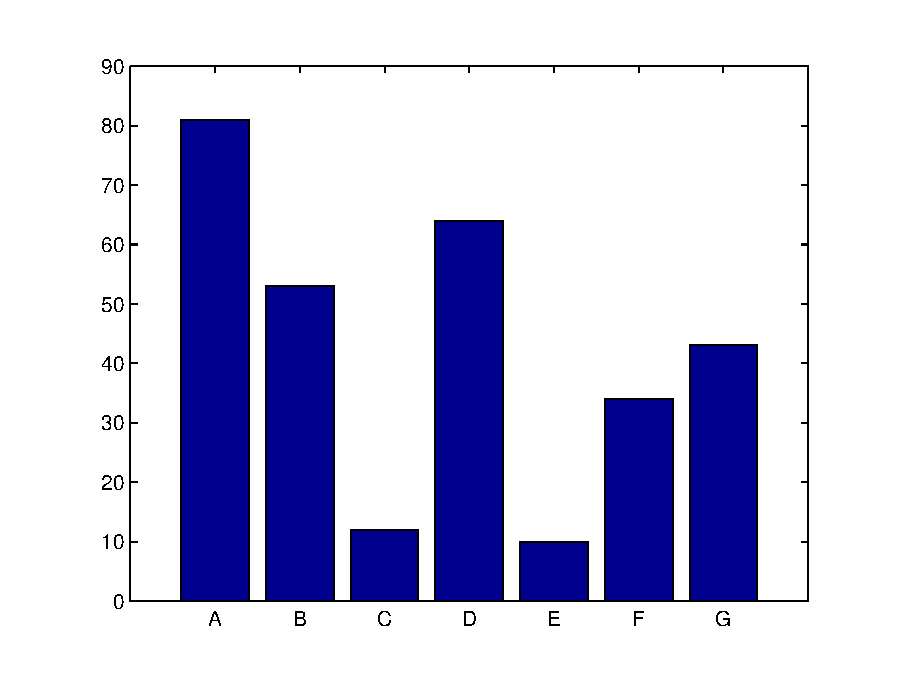
\includegraphics[width=\linewidth]{slike/bar_imenovan.eps}
\caption{Primjer stupčastog grafa sa proizvoljnim imenima stupaca.}
\label{fig:bar_imenovan}
\end{figure}

%\clearpage
%\listoffigures

\end{document}